\chapter{Using Single Board Heater System, Virtually!}\label{virtual}
\section{Introduction to Virtual Labs at \\IIT Bombay}
The concept of virtual laboratory is a brilliant step towards strengthening the education system of an university/college, a metropolitan area or even an entire nation. The idea is to use the ICT i.e. Information and Communications Technology, mainly the Internet for imparting education or exchange of educational information. Virtual Laboratory mainly focuses on providing the laboratory facility, virtually. Various experimental set-ups are hooked up to the internet and made available to use for the external world. Hence, anybody can connect to that equipment over the internet and carry out various experiments pertaining to it. The beauty of this idea is that a college who cannot afford to have some experimental equipments can still provide laboratory support to their students through virtual lab, and all that will cost it is a fair Internet connection! Moreover, the laboratory work does not ends with the college hours, one can always use the virtual lab at any time and at any place assuming the availability of an internet connection. 

A virtual laboratory for SBHS is launched at IIT Bombay. Here is the url to access it: {\bf vlabs.iitb.ac.in/sbhs/}. A set of 36 SBHS are made available to use over the internet 24$\times$ 7. These individual kits are made available to the users on hourly basis. We have a slot booking mechanism to achieve this. Since there are 36 SBHS connected with an hours slot for 24 hrs a day, we have 864 one hour slots a day. This means that 864 individual users can access the SBHS in a day for an hour. This also means that up to 6048 users can use the SBHS for an hour in a week and 181440 in a month! A web page is hosted which is the first interface to the user. The user registers/logs in himself/herself here. The user is also supposed to book a slot for accessing the SBHS. A database server maintains a record of the data generated through the web interface. A python script is hosted on the server side and it helps in connecting the user with the corresponding SBHS placed remotely. A free and open source scientific computing Software, Scilab, is used by the user for implementing the experiment on SBHS, in terms of simple Scilab coding. 

\section{Evolution of SBHS virtual labs}
In \cite{vlabs-kmm}, 
the control algorithm is implemented at the server end and the remote
student just keys in the parameters, as shown in Figure
\ref{fig:initial}. 
\begin{figure}
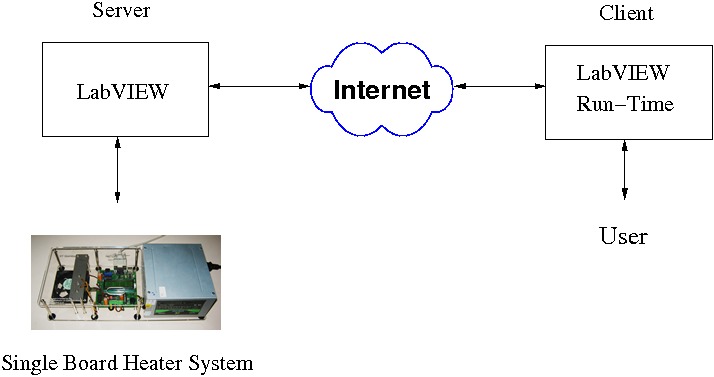
\includegraphics[width=\linewidth]{vlabs/vlab-1.png}
\caption{SBHS virtual laboratory with remote access using LabVIEW}
\label{fig:initial}
\end{figure}
LabVIEW was used for the implementation of the same. The
server end consisted of a computer connected with an SBHS with a full
blown copy of LabVIEW installed on it. The client has a LabVIEW run
time engine available for free download from the National Instruments
website.  A few
LabVIEW algorithms/experiments were hosted on the server. The client
accesses these algorithm/experiment over the Internet using a web
browser by entering appropriate parameters.

It was realized that the learning experience is not complete for this
structure. This is because the server hosts some pre-built LabVIEW
algorithms and a user can only access these few algorithms. The user
can in no way change the program and can only input experimental
parameters. 
Hence, we came up with a new architecture
as shown in the Figure \ref{fig:second} that used full blown copies of
LabVIEW at both server and client ends.  
\begin{figure}
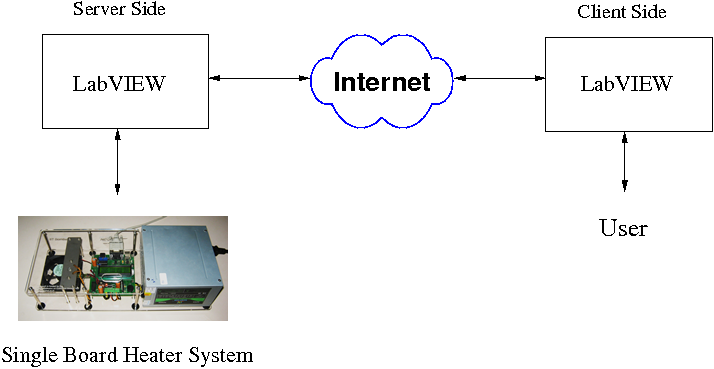
\includegraphics[width=\linewidth]{IEEE-Chile/figures/vlab-2.png}
\caption{SBHS virtual laboratory with remote access and live data sharing using LabVIEW}
\label{fig:second}
\end{figure}
 
 This idea uses the DataSocket technology of LabVIEW. Since now the
 client is having a complete LabVIEW installation on his/her computer
 she can now implement her own algorithms.  Thus this architecture did
 provide a complete learning experience to the students.  There are
 some shortcomings as well:

\begin{itemize}
\item LabVIEW is expensive and students may not be able to afford to
  buy it.  It is also prohibitively expensive for the Government to
  distribute it.

\item We used the LabVIEW version 8.04, which had restricted scripting
  language.  It was tedious to create new control algorithms in it.
\end{itemize}
\begin{figure}
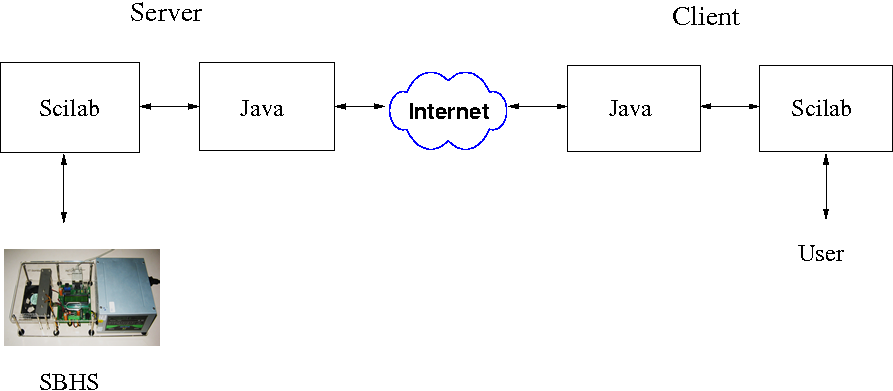
\includegraphics[width=\linewidth]{vlabs/vlab-3.png}
\caption{SBHS virtual laboratory using open source software}
\label{fig:third}
\end{figure}
This made us shift to free and open source (FOSS) software. We
replaced LabVIEW with Java and Scilab as shown in Figure
\ref{fig:third}. Scilab at the server end is used for communicating
with SBHS. Scilab at the client end is used for implementing the
algorithms. Java is used at both the server as well as client end for
communication over the Internet thereby connecting the client with the
server. 

For the above solution, we need a dedicated copy of scilab running at
the server end for every SBHS. One way to do this is to host it on
multiple computers with unique IPs. Hence the number of SBHS we want
to host requires as many computer's and public IPs thereby making
it expensive. Moreover, it also limits its scalability. The other way
to do this is to host multiple java and scilab servers on the same
computer.  Hosting many copies of Scilab simultaneously requires a
powerful computer for the server.

For these reasons  we decided to take scilab off the server computer
and to use java alone to communicate with the SBHS directly.  Java
also 
communicates with the client computer.  We connected seven SBHS
systems to a USB port through a serial port hub.  This architecture
was 
implemented on a Windows Operating System.  We faced the following
difficulties in this solution.
\begin{itemize}
\item When we connected more than one serial hub to a PC, the port ID
  could not be retrieved correctly.  Port ID information is required
  if we want a student to use the same SBHS for all their experiments
  during different sessions.
\item The experiments required time stamping of the data communicated
  to and from the server. But this time stamping was not linear and
  suffered instability.  
\end{itemize}
This made us to completely switch to FOSS with Ubuntu Linux as the OS
and is the current structure of the Virtual lab as shown in Figure
\ref{fig:detail-arch} 

\begin{figure}
\centering
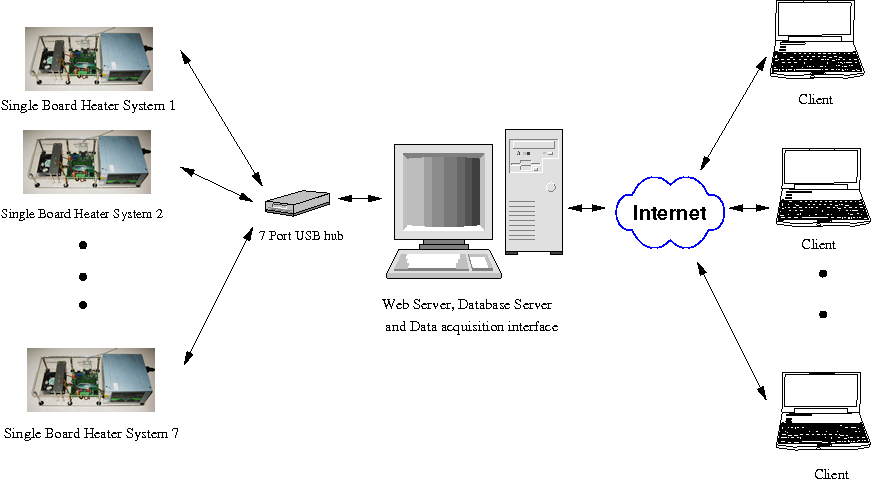
\includegraphics[width=\linewidth]{vlabs/vlab-arch}
\caption{Virtual control lab hardware architecture}
\label{fig:hw-arch}
\end{figure}

\section{Current Hardware Architecture}
The current hardware architecture of the virtual single-board heater system lab involves 36 single-board heater systems connected to the server via multiple 7 and 10-port USB hubs. The server computer is connected to a high speed internetwork and has enough processing capability to host data acquisition, database, and web servers. 
It has been successfully tested for the undergraduate Process Control course and the graduate Digital Control and Embedded systems courses conducted at IIT Bombay as well as few workshops over the internet. Currently, this architecture is integrated with a cameras on each SBHS to facilitate live video streaming. This gives the user a feel of remote hands-on. 

\section{Current Software Architecture} \label{sec:vlabarchi}
The current software architecture of this virtual SBHS control lab is shown in Figure \ref{fig:detail-arch}. The server computer runs Ubuntu Linux 12.04.2 OS. It hosts a Apache-MySQL server. The SBHS server is based on Python-Django framework and is linked to Apache server using Apache's WSGI module. The MySQL database server has the details of all the registered users, their slot details, authentication keys to allow remote access, etc. As shown in Figure \ref{fig:sbhs-website}, the Python-Django server has pages for registration, login, slot booking etc. \cite{vl010}.  On the client end, control algorithms are running in Scilab and a python based client application communicates with virtual labs server over the Internet.



\begin{figure}
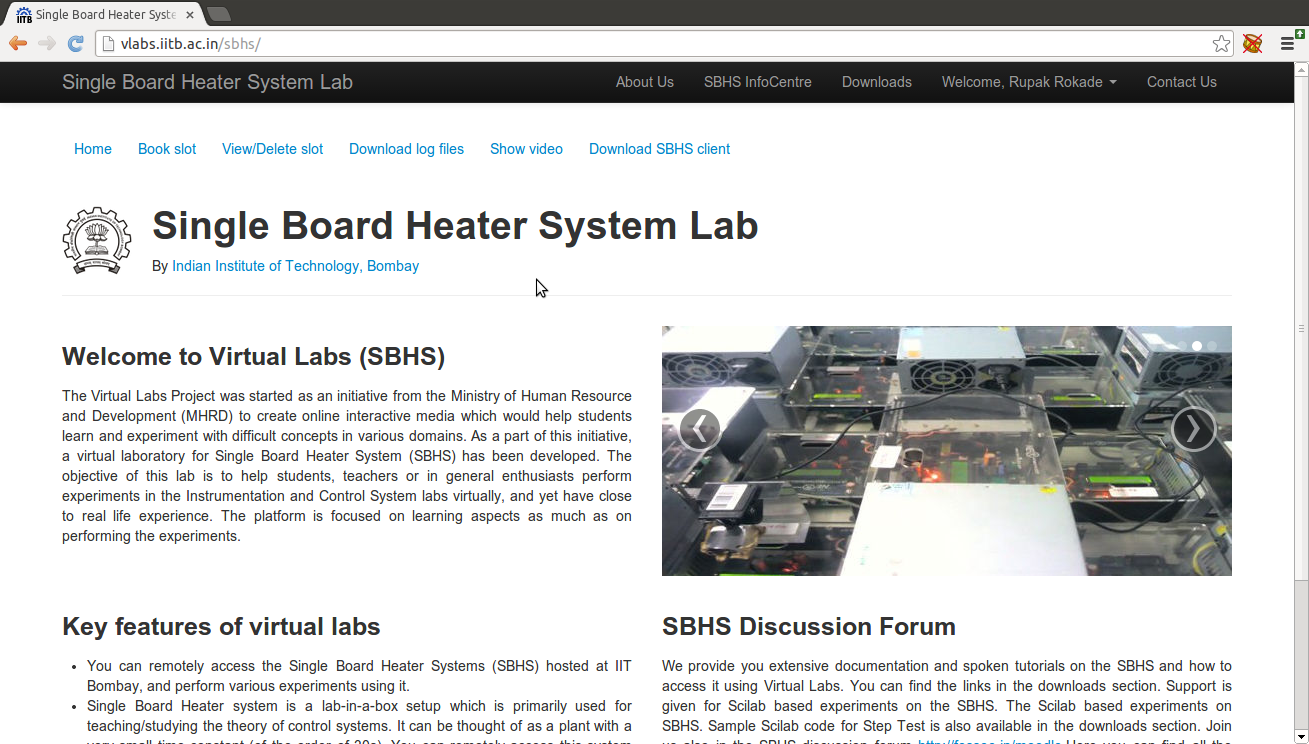
\includegraphics[width=\linewidth]{vlabs/webpage}
\caption{Home page of SBHS V Labs}
\label{vlabs-home}
\end{figure}
The steps to be performed before and during each experiment are explained next.

\begin{figure}
\centering
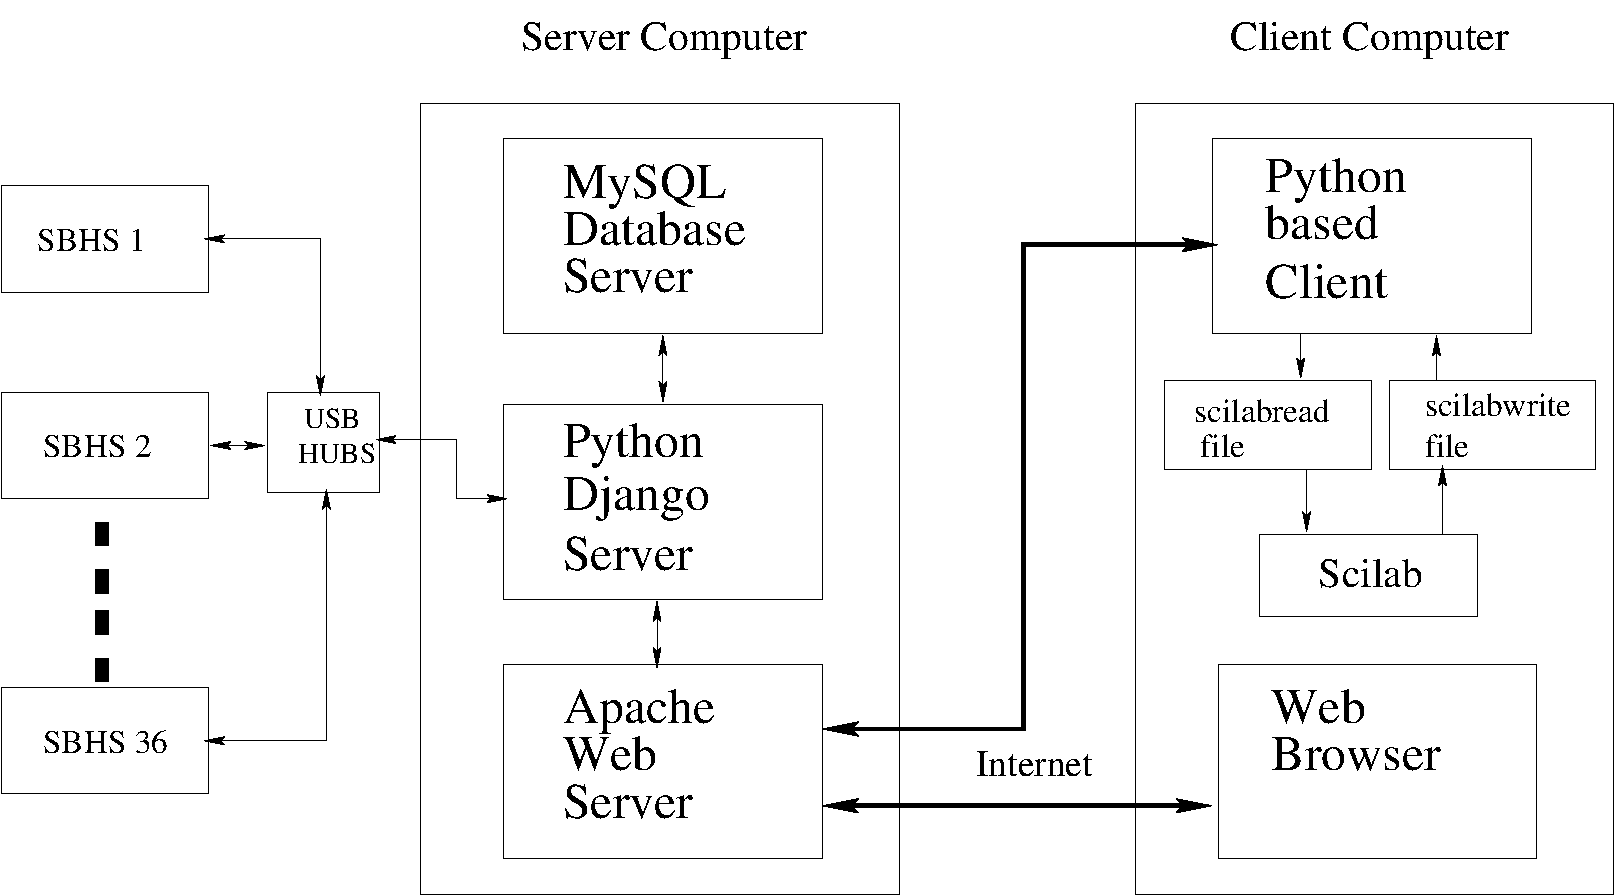
\includegraphics[width=\linewidth]{vlabs/new-server-arch.pdf}
\caption{Current Architecture of SBHS Virtual Labs}
\label{fig:detail-arch}
\end{figure}

\section{Conducting experiments using the Virtual lab}\label{vlabsexpt}

This section explains the procedure to use Single Board Heater System remotely using Scilab i.e. when you are accessing SBHS remotly using your computer over the virtual labs platform. An open loop experiment, step test is used for demonstrating this procedure. The process however remains the same for performing any other experiment explained in this section, unless specified otherwise. Let us first see the required files to be downloaded and installations to be done. Scilab is required to be installed on your computer. Please refer to Section \ref{driver} and Section \ref{linux-sbhs} for the procedure to install scilab on Windows and Linux system, respectively.

SBHS scilab code for your OS,  under the section {\tt SBHS Virtual Code}, must be downloaded from {\tt http://sbhs.os-hardware.in/downloads}. For example, if you are using a 32-bit linux operating system then you should download the file {\tt SBHS Scilab codes for Linux - (32 bit)}. The code downloaded will be in zip format. After the zip is unpacked, you will see scilab experiment folders such as {\tt Step\_test}, {\tt Ramp\_Test}, {\tt pid\_controller} etc. We will be using the {Step\_test} folder. Do not alter the directory structure. If you want to copy or move an experiment outside the directory then make sure you also copy the {\tt common\_files} folder. The {\tt common\_files} folder must always be one directory outside the experiment folder. Now given that you have scilab installed and working and the required scilab code downloaded, let us see the step-by-step procedure to do a remote experiment.

\subsection{Registration, Login and Slot Booking}\label{regAndslot}
 Go to the website {\tt sbhs.os-hardware.in} and click on the {\tt Virtual labs} link available on the left hand side. The home page of Virtual labs is illustrated in Fig \ref{vlabs-home}. If you are a first time user, click on the link {\tt Login/Register}. Fill out the registration form and submit it. If the registration form is submitted successfully, you will receive an activation link on your registered Email id. Use this link to complete the registration process. If you skip this step you will not be able to login. Registration is a one time process and need not be repeated more than once. After completing registration login with your username and password. You should now get the options to Book Slot, Delete Slot etc. 

View/Delete slot option allows you to delete your booked slots. This option however will work only for slots booked for the future. You cannot delete a past or the current slot. Download log files option gives you the facility to download your experiment log files. Clicking on it will give you a list of all of the experiments you had performed. Show video option can be used to see the live video feed of your SBHS. Web cameras are mounted on every SBHS. You can see the display of your SBHS as shown in Fig. \ref{web-cam}.

\begin{figure}
\centering
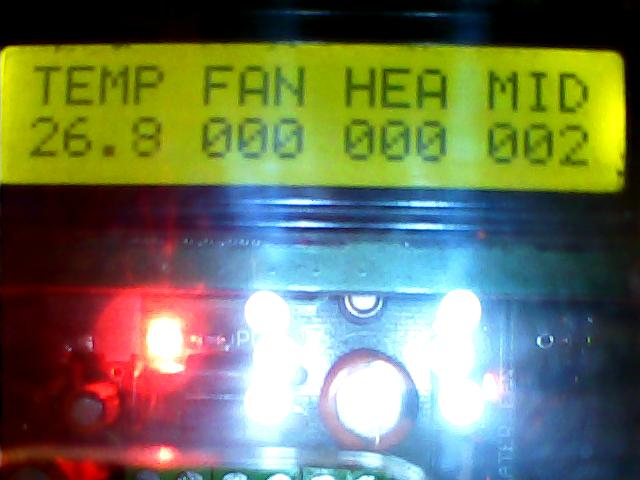
\includegraphics[width=0.5\linewidth]{vlabs/display.jpg}
\caption{Show Video}
\label{web-cam}
\end{figure}

Clicking on the Book slot option will allow you to book an experiment time slot. Slots are of 55 minutes duration. Click on the Book slot option. If the current slot is free, Book now option will appear. Click on it. Else you have to book an advance slot for the next hour or any other future time using the calender that appears on this page. There is a limit to how many slots one can book in a day. We are allowing only two non-consecutive slots, per user, to be booked in a day. However, there is no limit to how many current slots you book and use. Book an experiment slot. Once you successfully book a slot a {\bf Slot booked successfully} message highlighted in green color will appear on the top side. This is shown in Fig. \ref{book-slot}. It will automatically take you to the View/Delete slot page.

\begin{figure}
\centering
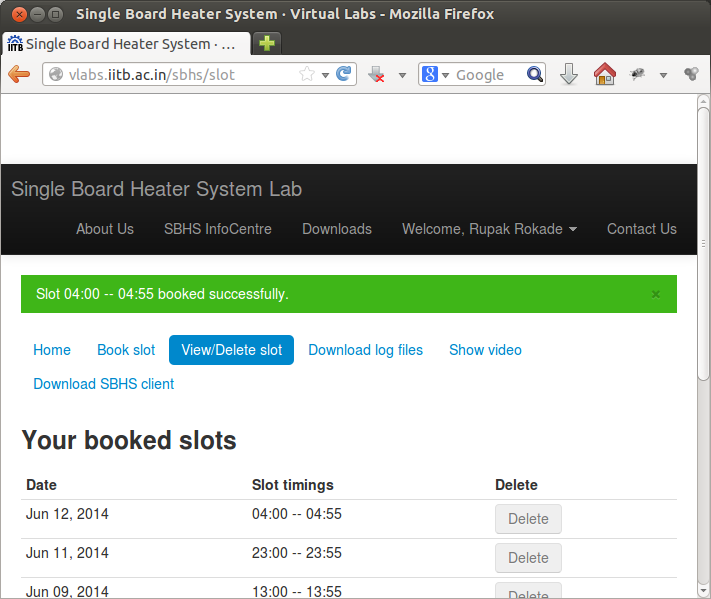
\includegraphics[width=0.7\linewidth]{vlabs/book-slot.png}
\caption{Slot booking}
\label{book-slot}
\end{figure}

\subsection{Configuring proxy settings and executing python based client}\label{proxy}
After booking a slot, the web activity is over. You may close the web browser unless you need it open to see live video feed of your SBHS. The next step is to establish the communication link between the server and your computer. A python based application is created which handles the network communication. 

Let us first see how to do the proxy  settings if you are behind a proxy network. Open the folder {\tt common\_files}. Open the file {\tt config}. This files contains various arguments whose values must be eneterd to configure proxy. 

{\bf Do not change the contents of {\tt config} file if}
\begin{itemize}
\item You are accessing from inside IIT Bombay OR
\item You are accessing from outside IIT Bombay and using an open network such as at home OR using a mobile internet
\end{itemize}

{\bf Change the contents of {\tt config}  file if}
\begin{itemize}
\item You are outside IIT Bombay and using a proxy network such as at an institute, office etc.
\end{itemize}

If you have to put the proxy details, first change the argument {\tt use\_proxy} = Yes (Y should be capital in Yes and N should be capital in No). Fill in the other details as per your proxy network. If your proxy network allows un-authenticated login then make the argument {\tt proxy\_username} and {\tt proxy\_password}  blank. This proxy setting has to done only once.

Open the {\tt Step\_test} folder. Double click on the file {\tt run}. This will open the client application as shown in Fig. \ref{python-client}. Note that for first time execution, it will take a minute to open the client application. It will show various parameters related to the experiment such as SBHS connection, Client version, User login and Experiment status. The green indicators show that the corresponding activity is correct or functional. Here it says that the Client application is been able to connect to the server and the client version being used is the latest. The User login and Experiment status is showing red and will turn green after a registered username and password is entered. If the SBHS is offline or there are some other issues, the corresponding error will be displayed and the respective indicator will turn red. Enter your registered username and password and press login. You should get the message {\tt Ready to execute scilab code}. The application also shows the value of iteration, heat, fan, temperature and time remaining for experimentation. It also shows the name of log file created for the experiment.

\begin{figure}
\centering
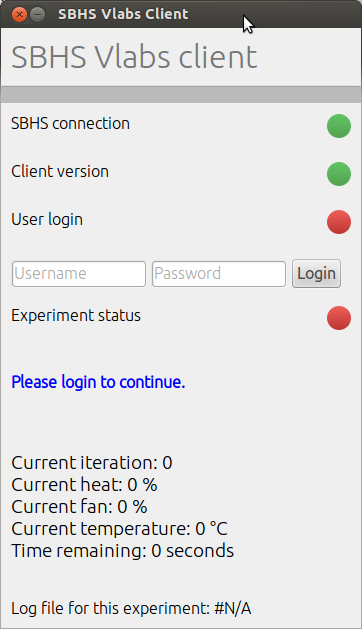
\includegraphics[width=0.5\linewidth]{vlabs/python-client.png}
\caption{Python Client}
\label{python-client}
\end{figure}


\subsection{Executing scilab code}
Inside the {\tt StepTest} folder, if on a windows system, double click on the  file {\tt stepc.sce}. This should automatically launch scilab and also open the {\tt stepc.sce} in the scilab editor. It will also automatically change the scilabs working directory. On a linux system, launch scilab manually. Then change the scilab working directory to the folder {\tt StepTest}. This can be done by clicking on {\tt File} menu and then selecting {\tt change current directory}. Next, execute the command {\tt getd ..\slash common\_files}. Scilab command {\tt getd} is used to load all functions defined in all .sci files inside a specified folder. Here we have some important function files inside the {\tt ..\slash common\_files} directory. Executing this command will load all of the functions that the experiment needs. Open the file {\tt stepc.sce} using the {\tt Open} option inside {\tt File} menu. The file is shown in Fig. \ref{stepc}

\begin{figure}
\centering
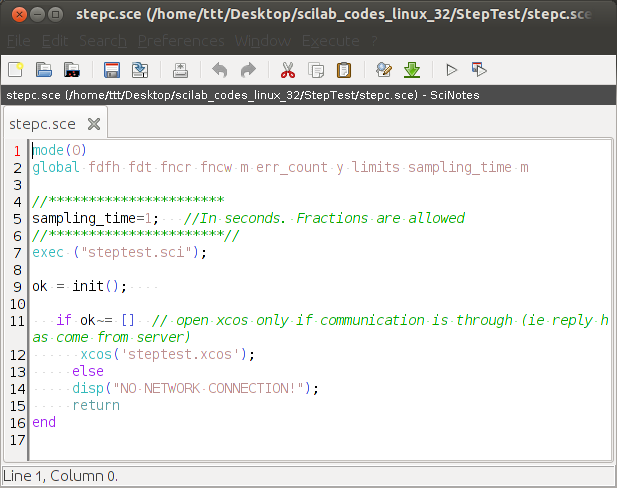
\includegraphics[width=0.7\linewidth]{vlabs/stepc.png}
\caption{stepc.sce file}
\label{stepc}
\end{figure}

The experiment sampling time can be set inside the  {\tt stepc.sce} file. You may want to change it to a higher value if your network is slow. The default value of 1 second works fine in most cases. On the menu bar, click on {\tt Execute} option and choose option {\tt file with echo}. This will execute  the scilab code. If the network is working fine, an xcos diagram will open automatically. If it doesnt open then see the scilab console for error messages. If you get a {\tt No network connection} error message then try executing the scilab code again. The xcos diagram is for the step test experiment as shown in Fig. \ref{step-xcos}. You can set the value of the heat and fan. Keep the default values. On the menu bar of the xcos window, click on {\tt start} button. This will execute the xcos diagram. If there is no error, you will get a graphic window with three plots. It will show the value of Heat in \% Fan in \% and ..temperature in degree celcius as shown in Fig. \ref{step-plot}. After sufficient time of experimentation click on the stop button to stop the experiment. Go to the {\tt StepTest} folder. Here you will find a {\tt logs} folder. This folder will have another folder named after your username. It will have the log file for your experiment. Read the log file name as\\ YearMonthDate\_hours\_minutes\_seconds.txt. This log file contains all the values of heat fan and temperature. It can be used for further analysis.

\begin{figure}
\centering
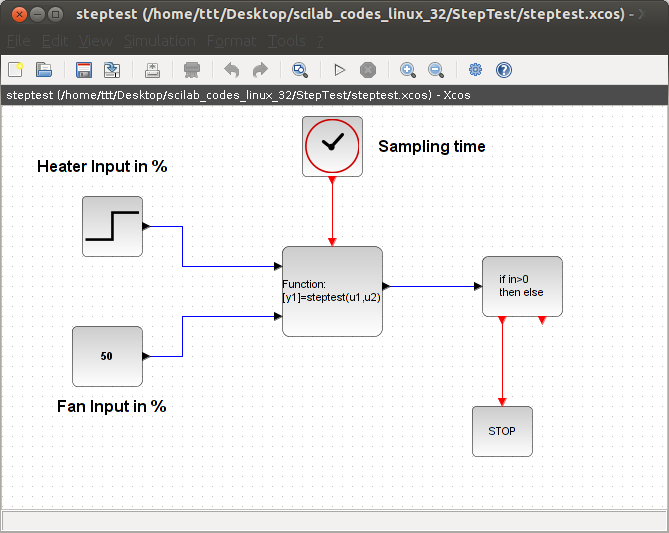
\includegraphics[width=0.7\linewidth]{vlabs/step-xcos.png}
\caption{Xcos for step test}
\label{step-xcos}
\end{figure}

\begin{figure}
\centering
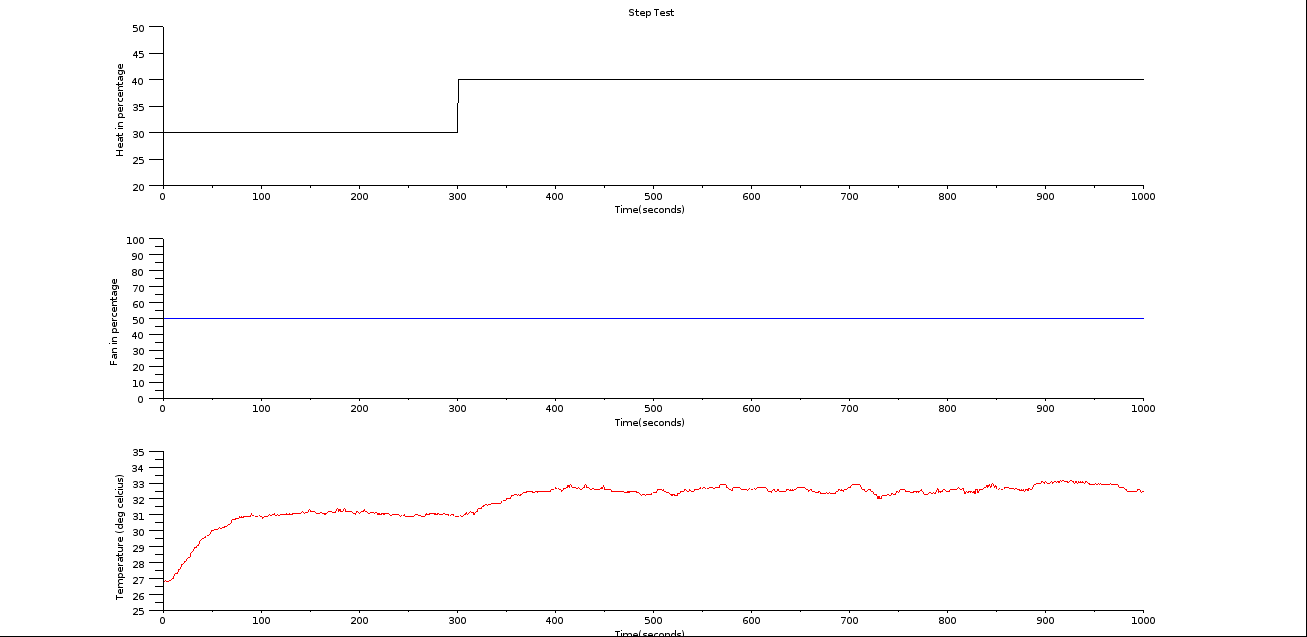
\includegraphics[width=0.7\linewidth]{vlabs/step-test-output.png}
\caption{Output of Step Test}
\label{step-plot}
\end{figure}

\subsection{Conducting experiments over virtual labs through ARM based computer}
This section talks about accessing the SBHS virtual labs using an ARM based computer. These ARM based computers could be netbooks, laptops or even tablets running a Linux operting system. Let us see the additional steps to be follwed for using over an ARM computer.
\begin{enumerate}
\item The scilab codes are separate for windows, linux and ARM based linux. Download the scilab code from {\tt http://sbhs.os-hardware.in/downloads}. You need to download the file against the label {\tt SBHS Scilab codes for ARM} under the {\tt SBHS Virtual Code} section. The name of the file downloaded will be {\tt sbhs\_codes\_arm}. This will be a zip file. Extract its connets in order to use it.
\item Open a terminal by pressing the {\tt Alt+Ctrl+T} keys together. Change the directory to {\tt sbhs\_codes\_arm} directory using the {\tt cd} command. For example, if the {\tt sbhs\_codes\_arm} folder is saved on the desktop, the command will look like {\tt cd Desktop/sbhs\_codes\_arm}
\item Execute the command {\tt chmod +x install.sh} 
\item Then execute the command {\tt ./install.sh}. It may ask you to enter the sudo password. Hence, this step requires you to know the sudo password of the computer you are using.
\item With these steps done, now follow the instructions explained in Section \ref{vlabsexpt} throughout its subsections. Note that you need NOT download {\tt SBHS Scilab codes for Linux - (32 bit)
} file while refering to this section. This is because all scilab codes are included inside the {\tt sbhs\_codes\_arm} directory
\end{enumerate}
\section{Summary}\label{virtual-summary}

This section summarizes the process to perform an experiment on SBHS using virtual lab interface. This section assumes that the user has already created an account and booked a slot as explained in section \ref{regAndslot}. It also assumes that the proxy settings are already done as explained in section \ref{proxy}. The user should follow these steps within the booked slot time.
\begin{itemize}
\item Step1: Open the StepTest experiment directory
\item Step2: Double-click on the file {\tt run}. Expect the SBHS cient application to open.
\item Step3: Enter the username and password inside the SBHS cient application and press {\tt login} button. Expect the message {\tt Ready to execute scilab code}
\item Step4: Switch to the StepTest experiment directory and double-click on the file {\tt stepc.sce}. This will launch scilab and also open the file {\tt stepc.sce} in the scilab editor. Linux users will have to launch scilab manually. They also have to change the working directory to StepTest and then open the {\tt stepc.sce} file in the scilab editor.
\item Step5 Switch to the scilab console and execute the command {\tt getd ..\slash common\_files}
\item Step6: Execute the file {\tt stepc.sce}. Expect the step test xcos diagram to open automatically. If this doesnt happen, check the scilab console for error message.
\item Step7: Execute the step test xcos daiagram. You may change the input parameters, if required, before executing. Expect a plot window to open automatically showing three graphs.
\item Step8: Stop the Xcos simulation after the experiment is completed properly. 

\end{itemize}